\documentclass[11pt,letterpaper]{article}

\usepackage[T1]{fontenc}
\usepackage[utf8]{inputenc}
\usepackage{lmodern}
\usepackage{microtype}
\usepackage{amsmath,amssymb,amsthm}
\usepackage[margin=1in]{geometry}
\usepackage{tikz}
\usepackage{fancyhdr}
\usepackage{xcolor}
\usepackage[colorlinks=true,linkcolor=blue!60!black,citecolor=blue!60!black,urlcolor=blue!60!black]{hyperref}
\usepackage{bookmark}

\setlength{\parskip}{0.35em}
\setlength{\emergencystretch}{3em}
\setlength{\headheight}{14pt}
\pagestyle{fancy}
\fancyhf{}
\fancyhead[L]{\small Erd\H{o}s Problem 289}
\fancyhead[R]{\small J. Land}
\fancyfoot[C]{\thepage}
\renewcommand{\headrulewidth}{0.3pt}
\fancypagestyle{plain}{\fancyhf{}\fancyfoot[C]{\thepage}\renewcommand{\headrulewidth}{0pt}}

\numberwithin{equation}{section}
\theoremstyle{plain}
\newtheorem{theorem}{Theorem}
\newtheorem{corollary}{Corollary}
\newtheorem{proposition}{Proposition}
\newtheorem{lemma}{Lemma}
\theoremstyle{remark}
\newtheorem{remark}{Remark}

\newcommand{\N}{\mathbb N}
\newcommand{\Z}{\mathbb Z}
\newcommand{\Q}{\mathbb Q}
\newcommand{\cP}{\mathcal P}
\newcommand{\cF}{\mathcal F}
\newcommand{\cU}{\mathcal U}
\newcommand{\cR}{\mathcal R}
\newcommand{\cA}{\mathcal A}
\newcommand{\cC}{\mathcal C}
\newcommand{\cM}{\mathcal M}
\newcommand{\lcm}{\operatorname{lcm}}
\newcommand{\core}{\mathrm{core}}
\newcommand{\main}{\mathrm{main}}

\hypersetup{pdftitle={A solution of Erdős Problem 289 with intervals of length two and three},
  pdfauthor={Johan Land}}

\title{A solution of Erd\H{o}s Problem 289\\ with intervals of length two and three}
\author{Johan Land\\ \small Independent Researcher}
\date{4 September 2026}

\begin{document}
\maketitle

\begin{abstract}
Erd\H{o}s and Graham asked whether, for every sufficiently large integer $k$, there exist $k$ finite intervals of positive integers, each containing at least two integers and no two of them overlapping or adjacent, such that the reciprocals of all integers in the intervals sum to $1$. We prove a stronger statement: for every sufficiently large $k$ the intervals can be chosen to have length two or three and to lie in $[1,20k]$. The proof combines the Bourgain--Garaev bound for short sums of modular inverses, the structure theorem of Conlon, Fox, He, Mubayi, Pham, Suk and Verstra\"ete for subset sums, and the Liu--Sawhney density theorem for unit fractions, with a descent through the prime powers of a denominator that cancels one prime power at a time using pairs of consecutive integers while adding a predetermined number of intervals at every stage.
\end{abstract}

\section{Introduction}\label{sec:intro}

\subsection{The problem and the main theorem}\label{sec:problem}

Problem 289 on the Erd\H{o}s problems site \cite{EP289}, originating in Erd\H{o}s and Graham \cite{EG80}, reads as follows.

\begin{quote}
Is it true that, for all sufficiently large $k$, there exist finite intervals $I_1,\ldots,I_k\subset\N$, distinct, not overlapping or adjacent, with $|I_i|\ge2$ for $1\le i\le k$, such that
\[
1=\sum_{i=1}^k\sum_{n\in I_i}\frac1n\,?
\]
\end{quote}

Throughout, an interval of integers $[a,b]$ with $a\le b$ consists of all integers $n$ with $a\le n\le b$, so $|[a,b]|=b-a+1$. Two intervals $[a,b]$ and $[a',b']$ with $b<a'$ are \emph{adjacent} if $b+1=a'$, and \emph{separated} if $b+1<a'$, that is, if at least one integer lies strictly between them. A family of intervals is separated if any two of its members are separated after ordering them.

\begin{theorem}\label{thm:main}
For every sufficiently large integer $k$ there are integer intervals $[a_i,b_i]$, $1\le i\le k$, such that
\begin{equation}\label{eq:main}
2\le a_i\le b_i\le20k,\qquad b_i-a_i+1\in\{2,3\},\qquad
b_i+1<a_{i+1}\ \ (1\le i<k),\qquad
\sum_{i=1}^k\sum_{n=a_i}^{b_i}\frac1n=1 .
\end{equation}
\end{theorem}

\begin{corollary}\label{cor:289}
The answer to Problem 289 is affirmative: for all sufficiently large $k$ there exist finite intervals $I_1,\ldots,I_k\subset\N$, distinct, not overlapping or adjacent, with $|I_i|\ge2$, such that $1=\sum_i\sum_{n\in I_i}1/n$.
\end{corollary}

\begin{proof}
Take $I_i=[a_i,b_i]$ from Theorem~\ref{thm:main}. For $i<j$ the inequalities $b_i+1<a_{i+1}\le a_j$ show that $I_i$ and $I_j$ are disjoint, hence distinct, and that the integer $b_i+1$ lies in neither of them, so they are not adjacent. Each $|I_i|\in\{2,3\}$ is at least $2$, and the reciprocal sum is the same.
\end{proof}

The separation requirement is the substance of the problem. If adjacent intervals were permitted, any interval of length at least four could be cut into adjacent pieces of lengths two and three, so the number $k$ of intervals would carry no information; and as observed in the discussion of \cite{EP289}, without the restrictions the question is easy. Theorem~\ref{thm:main} says more than the problem asks: the intervals have length two or three, and all of them lie in $[1,20k]$. The constant $20$ is not optimized; it arises from the far band $[4k,20k]$ used in Section~\ref{sec:main}, where the only requirement is the inequality $16\gamma>1$ in \eqref{eq:gammabounds}.

\subsection{Outline of the proof}\label{sec:outline}

The proof adapts the absorption argument in Section~4 of Conlon, Fox, He, Mubayi, Pham, Suk and Verstra\"ete \cite{CFHMPSV}. Its descending cancellation of denominator prime powers, its small reciprocal budget, and its terminal reservoir form the starting architecture. Lemma~\ref{lem:cover} below is a sparse version of that paper's inverse-covering theorem, proved by the same bounded-rank progression and divisor-count method. The new ingredients are powersmooth consecutive-pair fibers, the separation of those pairs, a fixed number of pairs at each correction stage, and a core completed by extending pairs to triples.

The final family consists of intervals of three kinds, living at three different scales (Figure~\ref{fig:line}).

\begin{enumerate}
\item \textbf{Core pairs} $[Kd+1,Kd+2]$, where $K$ is a fixed integer and $d$ runs over a set $\cR$ of parameters of size $\Theta(k^{4/5})$ (Section~\ref{sec:core}). Some of these pairs will later be extended to the triples $[Kd,Kd+2]$.
\item \textbf{Main pairs} $[a,a+1]$ with $3\mid a$, lying in $[k/1024,k]\cup[4k,20k]$, all of whose endpoints are $k^{4/5}$-powersmooth (Section~\ref{sec:main}). There are exactly $k-|\cR|-C_H$ of them, where $C_H$ is a number fixed in advance, and they are chosen so that the \emph{initial deficit}
\[
r_0=1-(\text{mass of core})-(\text{mass of main pairs})
\]
is a rational number of size about $\delta/2$, with $\delta=1/1000$, whose denominator has all prime-power divisors at most $H=O(k^{4/5})$.
\item \textbf{Correction and auxiliary pairs} at scale between $L^{11/10}$ and $O(k^{22/25})$, added by a descent (Section~\ref{sec:descent}) which cancels the prime powers of the denominator of $r_0$ one at a time, in decreasing order.
\end{enumerate}

The descent works as follows. Let $q=p^a$ be the largest prime power in the current denominator. Lemma~\ref{lem:fiber} supplies a \emph{fiber} $I_q$ of about $q^{\varepsilon}$ integers $m$ such that $qm+1$ has only prime-power divisors below $q/2$. The mass of the pair $[qm,qm+1]$ is
\[
w(qm)=\frac1{qm}+\frac1{qm+1},
\]
and modulo $q$ the first term behaves like $m^{-1}/q$ while the second is a junk term whose denominator involves only smaller prime powers. Lemma~\ref{lem:cover} shows that the inverses of a sparse set of size $q^{7\varepsilon/8}$ already cover every residue modulo $q$ using at most $q^{\varepsilon/2}$ summands. Subtracting the corresponding pair masses therefore removes the factor $p^a$ from the denominator while introducing only smaller prime powers. This is the obstacle peculiar to pairs, as opposed to single unit fractions: the junk term $1/(qm+1)$ must not reintroduce large prime powers, which is exactly what powersmoothness of $qm+1$ guarantees.

To make the total number of intervals predetermined, Lemma~\ref{lem:aux} reserves, for each prime power $q$, a family $\cF_q$ of exactly $s(q)=\lfloor q^{1/20}\rfloor$ \emph{auxiliary} pairs whose endpoints are $(q/2)$-powersmooth. If the cancellation at $q$ uses $c\le s(q)$ correction pairs, $s(q)-c$ auxiliary pairs are added as well. Every stage then adds exactly $s(q)$ intervals, and the whole descent adds exactly $C_H=\sum_{L<q\le H}s(q)$ intervals. No interval is ever split or merged.

After the descent the residual deficit is $j/K$ for some integer $1\le j\le j_0$, with $j_0$ fixed. It is absorbed by extending core pairs to triples: extending $[Kd+1,Kd+2]$ to $[Kd,Kd+2]$ adds $1/(Kd)$, and the Liu--Sawhney theorem (through Lemma~\ref{lem:dense}) supplies, inside each of $j$ disjoint bands of parameters, a set $D$ with $\sum_{d\in D}1/d=1$. This adds exactly $j/K$ without changing the number of intervals.

Separation is arranged by construction at each scale: correction pairs start at multiples of four (Lemma~\ref{lem:sep}), auxiliary pairs are chosen at distance at least two from every possible correction endpoint (Lemma~\ref{lem:aux}), core parameters $d$ are only used when the neighbourhood $[Kd-1,Kd+3]$ avoids every correction and auxiliary endpoint, and main pairs lie on a grid of spacing three, far beyond every other endpoint. The final assembly in Section~\ref{sec:proof} only verifies the count, the mass and the conditions in \eqref{eq:main}. Figure~\ref{fig:deps} shows how the ingredients depend on one another.

\begin{figure}[ht]
\centering
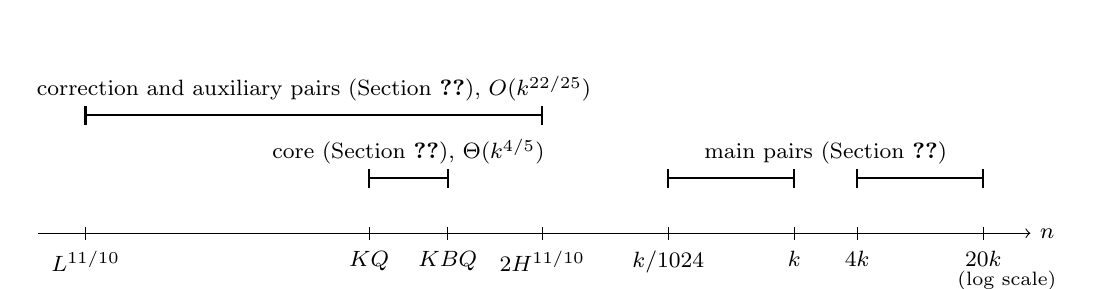
\begin{tikzpicture}[x=1cm,font=\footnotesize]
\draw[->] (0,0) -- (12.6,0) node[right] {$n$};
\node[below,font=\scriptsize] at (12.3,-0.35) {(log scale)};
\newcommand{\tick}[2]{\draw (#1,-0.08) -- (#1,0.08); \node[below] at (#1,-0.1) {#2};}
\tick{0.6}{$L^{11/10}$} \tick{4.2}{$KQ$} \tick{5.2}{$KBQ$} \tick{6.4}{$2H^{11/10}$}
\tick{8.0}{$k/1024$} \tick{9.6}{$k$} \tick{10.4}{$4k$} \tick{12.0}{$20k$}
\draw[thick] (0.6,1.5) -- (6.4,1.5);
\draw[thick] (0.6,1.38) -- (0.6,1.62);
\draw[thick] (6.4,1.38) -- (6.4,1.62);
\node[above] at (3.5,1.55) {correction and auxiliary pairs (Section~\ref{sec:descent}), $O(k^{22/25})$};
\draw[thick] (4.2,0.7) -- (5.2,0.7);
\draw[thick] (4.2,0.58) -- (4.2,0.82);
\draw[thick] (5.2,0.58) -- (5.2,0.82);
\node[above] at (4.7,0.75) {core (Section~\ref{sec:core}), $\Theta(k^{4/5})$};
\draw[thick] (8.0,0.7) -- (9.6,0.7);
\draw[thick] (8.0,0.58) -- (8.0,0.82);
\draw[thick] (9.6,0.58) -- (9.6,0.82);
\draw[thick] (10.4,0.7) -- (12.0,0.7);
\draw[thick] (10.4,0.58) -- (10.4,0.82);
\draw[thick] (12.0,0.58) -- (12.0,0.82);
\node[above] at (10.0,0.75) {main pairs (Section~\ref{sec:main})};
\end{tikzpicture}
\caption{Where the three kinds of intervals live. Here $Q=\lfloor k^{4/5}\rfloor$, $H=KBQ+2$, and $K$, $B$, $L$ are constants.}\label{fig:line}
\end{figure}

\begin{figure}[ht]
\centering
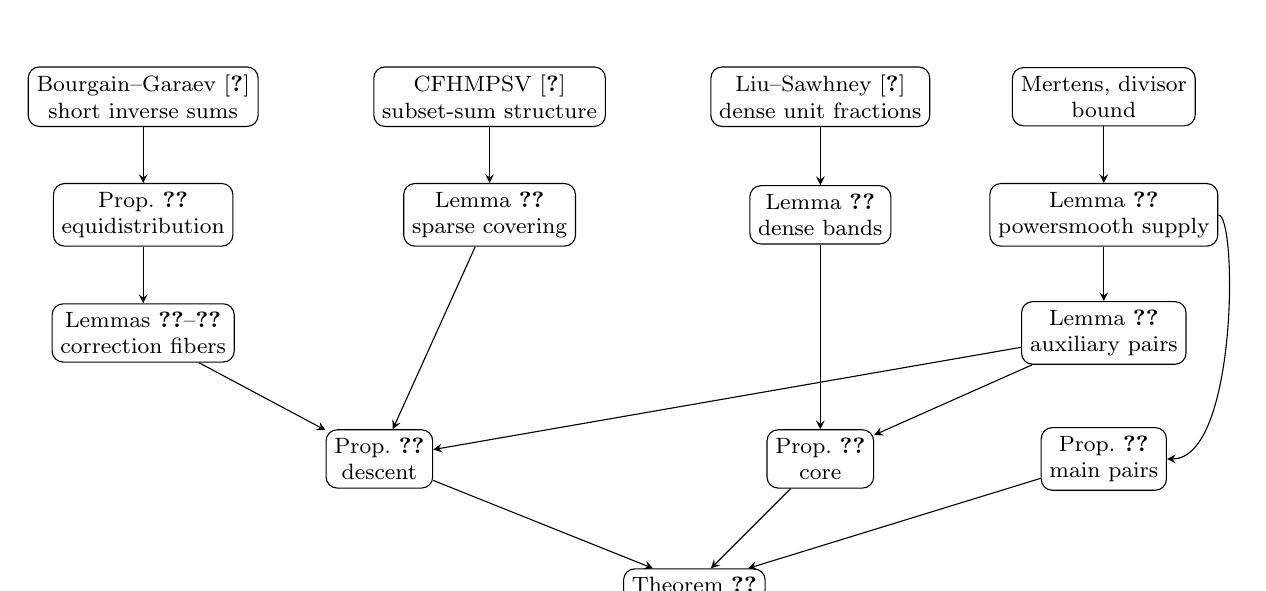
\begin{tikzpicture}[font=\footnotesize, every node/.style={draw, rounded corners, inner sep=3pt, align=center}, >=stealth]
\node (BG) at (0,3.2) {Bourgain--Garaev \cite{BG}\\ short inverse sums};
\node (CF) at (4.4,3.2) {CFHMPSV \cite{CFHMPSV}\\ subset-sum structure};
\node (LS) at (8.6,3.2) {Liu--Sawhney \cite{LS}\\ dense unit fractions};
\node (EL) at (12.2,3.2) {Mertens, divisor\\ bound};
\node (P1) at (0,1.7) {Prop.~\ref{prop:equi}\\ equidistribution};
\node (L3) at (4.4,1.7) {Lemma~\ref{lem:cover}\\ sparse covering};
\node (L6) at (8.6,1.7) {Lemma~\ref{lem:dense}\\ dense bands};
\node (L4) at (12.2,1.7) {Lemma~\ref{lem:supply}\\ powersmooth supply};
\node (L1) at (0,0.2) {Lemmas~\ref{lem:fiber}--\ref{lem:sep}\\ correction fibers};
\node (L5) at (12.2,0.2) {Lemma~\ref{lem:aux}\\ auxiliary pairs};
\node (P3) at (3.0,-1.4) {Prop.~\ref{prop:descent}\\ descent};
\node (P4) at (8.6,-1.4) {Prop.~\ref{prop:core}\\ core};
\node (P5) at (12.2,-1.4) {Prop.~\ref{prop:main}\\ main pairs};
\node (T) at (7.0,-3.0) {Theorem~\ref{thm:main}};
\draw[->] (BG) -- (P1); \draw[->] (P1) -- (L1); \draw[->] (CF) -- (L3); \draw[->] (LS) -- (L6);
\draw[->] (EL) -- (L4); \draw[->] (L4) -- (L5); \draw[->] (L6) -- (P4); \draw[->] (L4.east) .. controls (13.9,1.7) and (13.9,-1.4) .. (P5.east);
\draw[->] (L1) -- (P3); \draw[->] (L3) -- (P3); \draw[->] (L5) -- (P3); \draw[->] (L5) -- (P4);
\draw[->] (P3) -- (T); \draw[->] (P4) -- (T); \draw[->] (P5) -- (T);
\end{tikzpicture}
\caption{Dependencies among the main statements.}\label{fig:deps}
\end{figure}

\subsection{Notation and conventions}\label{sec:notation}

An integer is \emph{$y$-powersmooth} if every prime-power divisor of it is at most $y$. The largest prime-power divisor of an integer always refers to numerical size. For a positive integer $a$ and a modulus $m$ write
\[
w(a)=\frac1a+\frac1{a+1},\qquad e_m(x)=\exp(2\pi ix/m).
\]
The \emph{mass} of a set of pairwise disjoint intervals is the sum of the reciprocals of all integers in them; thus the pair $[a,a+1]$ has mass $w(a)$. All logarithms are natural, $\pi(x)$ counts primes up to $x$, and $\tau(n)$ is the number of divisors of $n$. A prime power is an integer $p^a$ with $p$ prime and $a\ge1$; sums and unions over $q$ ``prime power'' in a range run over all such integers in that range. Asymptotic notation $o(\cdot)$ and $O(\cdot)$ refers to $q\to\infty$ or $k\to\infty$, as indicated, with every constant of Section~\ref{sec:params} held fixed.

\subsection{Formal verification}\label{sec:formal}

A formalization of Theorem~\ref{thm:main} in Lean~4 with Mathlib is in progress \cite{Repo}. The formal target states \eqref{eq:main} for intervals indexed by $\{0,\ldots,k-1\}$ with separation required for every ordered pair of indices, exactly as in Theorem~\ref{thm:main}. We note that the formalization of Problem 289 in the Formal Conjectures library \cite{FC289} asks only for disjoint intervals and omits adjacency; Theorem~\ref{thm:main} implies both readings.

\section{External inputs and choice of parameters}\label{sec:inputs}

The proof uses three theorems from the literature. Each is stated here in the form in which it is used, together with the place where its hypotheses are verified.

\subsection{Short sums of modular inverses}\label{sec:BG}

\begin{theorem}[Bourgain--Garaev {\cite[Theorem 5]{BG}}]\label{thm:BG}
For every sufficiently small fixed $c>0$, as the integer modulus $m$ tends to infinity, uniformly in $m^c<N<m$ and in coefficients $a$ coprime to $m$,
\[
\Bigl|\sum_{\substack{n\le N\\ (n,m)=1}}e_m(an^{-1})\Bigr|=o(N).
\]
\end{theorem}

The quantitative bound in \cite{BG} is $N(\log\log m)^{O_c(1)}/\sqrt{\log m}$. Theorem~\ref{thm:BG} is used only in the proof of Proposition~\ref{prop:equi}, where it is converted into equidistribution of inverses in intervals by the Erd\H{o}s--Tur\'an inequality \eqref{eq:ET}.

\subsection{Structure in bounded subset sums}\label{sec:CF}

A generalized arithmetic progression of rank $D$ is a set of the form
\[
P=\Bigl\{\sum_{i=1}^Dn_id_i:\ \alpha_i\le n_i\le\beta_i,\ n_i\in\Z\Bigr\}
\]
with integer generators $d_i$ and real $\alpha_i\le\beta_i$; it is \emph{proper} if distinct coordinate vectors give distinct integers. The dilate $tP$ is defined in Section~\ref{sec:dilate}.

\begin{theorem}[Conlon--Fox--He--Mubayi--Pham--Suk--Verstra\"ete {\cite[Theorem 3]{CFHMPSV}}]\label{thm:CF}
Given fixed $\beta>1$ and $0<\eta<1$, there are constants $c>0$ and $d_0$ with the following property. If $A\subseteq[1,n]$, $|A|=m$, $n\le m^\beta$, and
\[
m^\eta\le s\le cm/\log_2m,
\]
then there are $J\subseteq A$, a proper generalized arithmetic progression $P$ of rank at most $d_0$, and $J'\subseteq J$, such that
\[
|J|\ge m-c^{-1}s\log_2m,\qquad J\cup\{0\}\subseteq P,\qquad |J'|\le s,
\]
and the subset sums of $J'$ contain a translate of the nonempty proper dilate $csP$, with dilation taken in the supplied representation.
\end{theorem}

This is derived in \cite{CFHMPSV} from Conlon--Fox--Pham \cite[Theorem 1.5]{CFP}. We cite the numbering of the journal version of \cite{CFHMPSV}, which agrees with arXiv version 2; the numbering differs in the first arXiv version. The logarithms in Theorem~\ref{thm:CF} are to base $2$, following the convention of \cite{CFP}; elsewhere in this paper logarithms are natural, and the change of base only affects the constant $c$. Theorem~\ref{thm:CF} is used only in the proof of Lemma~\ref{lem:cover}.

Two points about the dilate deserve comment. First, properness of a represented progression does not by itself imply that its dilate is nonempty: a proper coordinate box may contain no integer point after dilation by a noninteger factor. Nonemptiness is nevertheless part of what the source proves, because the representation supplied in the proof of \cite[Theorem 1.5, pp.~26--27]{CFP} is centered, and a centered coordinate box contains the zero vector after every positive dilation. Second, for noninteger $t$ the dilate $tP$ depends on the representation of $P$; the statement refers to the representation supplied there, which is kept fixed throughout.

\subsection{Dense sets contain a unit-fraction sum of one}\label{sec:LS}

\begin{theorem}[Liu--Sawhney {\cite[Theorem 1.3]{LS}}]\label{thm:LS}
For any fixed $0<\zeta<1/2$, every sufficiently large $N$ and every $A\subseteq[1,N]$ with
\[
|A|\ge(1-1/e+\zeta)N
\]
admit $D\subseteq A$ with $\sum_{d\in D}1/d=1$.
\end{theorem}

Theorem~\ref{thm:LS} is used only in the proof of Lemma~\ref{lem:dense}.

\subsection{Elementary estimates}\label{sec:elem}

We use Chebyshev's bound $\pi(x)\ll x/\log x$, Mertens' estimate
\begin{equation}\label{eq:mertens}
\sum_{p\le x}\frac1p=\log\log x+B_1+o(1)
\end{equation}
for a constant $B_1$, and the divisor bound $\tau(n)=n^{o(1)}$; see \cite[Theorems 7, 427 and 315]{HW}. We also use the Erd\H{o}s--Tur\'an inequality in the following form \cite[Chapter 1]{Mo}: there is an absolute constant $C_0$ such that for real numbers $x_1,\ldots,x_N$, every interval $J\subseteq[0,1)$ and every integer $T\ge1$,
\begin{equation}\label{eq:ET}
\Bigl|\#\{n\le N:\ \{x_n\}\in J\}-N|J|\Bigr|
\le C_0\Bigl(\frac NT+\sum_{h=1}^T\frac1h\Bigl|\sum_{n\le N}e(hx_n)\Bigr|\Bigr),
\end{equation}
where $\{x\}$ is the fractional part and $e(x)=\exp(2\pi ix)$.

\subsection{Choice of parameters}\label{sec:params}

All constants are chosen once, in the following order, and are independent of $k$.

\begin{enumerate}
\item $\varepsilon=1/10$. Lemmas~\ref{lem:fiber}, \ref{lem:sep} and \ref{lem:cover} are proved for every fixed $\varepsilon\in(0,1)$; only this value is used afterwards.
\item $\delta=1/1000$, the approximate size of the initial deficit.
\item An integer $L$, so large that: Lemmas~\ref{lem:fiber} and \ref{lem:cover} (with $\varepsilon=1/10$) hold for every prime power $q>L$; Lemma~\ref{lem:aux} holds for the cutoff $L$; and
\begin{equation}\label{eq:Lcond}
40L^{-1/20}<\delta/16,\qquad K:=\lcm(1,\ldots,L)\ \text{satisfies}\ K\delta\ge2\ \text{and}\ K\ge8.
\end{equation}
Each of these conditions holds for all sufficiently large $L$, so a single choice of $L$ meets all of them.
\item $K=\lcm(1,\ldots,L)$, $j_0=\lceil K\delta\rceil$, and $B=4^{j_0}$.
\item For every prime power $q>L$, a fiber $I_q$ from Lemma~\ref{lem:fiber} and a family $\cF_q$ of $s(q)=\lfloor q^{1/20}\rfloor$ auxiliary pairs from Lemma~\ref{lem:aux}. These determine the endpoint sets $\cP^*$, $\cF^*$ and $\cU=\cP^*\cup\cF^*$ of Section~\ref{sec:descent}.
\end{enumerate}

The quantities depending on $k$ are then determined in this order:
\begin{gather*}
Q=\lfloor k^{4/5}\rfloor,\qquad H=KBQ+2,\qquad
C_H=\sum_{\substack{L<q\le H\\ q\ \text{prime power}}}s(q),\\
\cR\ \text{and}\ R=|\cR|\ \text{(Section~\ref{sec:core})},\qquad M=k-R-C_H .
\end{gather*}
The phrase ``for sufficiently large $k$'' is used at finitely many places, each time with a threshold depending only on the constants above. The argument yields no explicit value of that threshold, and the constants $K$ and $B$, as well as the thresholds implicit in Theorems~\ref{thm:BG}--\ref{thm:LS}, are extremely large.

\section{Powersmooth fibers and correction pairs}\label{sec:fibers}

Throughout this section $q=p^a$ is a prime power tending to infinity, $0<\varepsilon<1$ is fixed, and $M=q^{\varepsilon}$. A \emph{correction pair} is a pair $[qm,qm+1]$ with $m$ in the fiber $I_q$ constructed in Lemma~\ref{lem:fiber}.

\subsection{Equidistribution of inverses in short intervals}\label{sec:equi}

We call an integer $t$ \emph{eligible} if $t$ is odd (in case $q=2^a$) or $(t,2p)=1$ (in case $q=p^a$ with $p$ odd). The density of eligible integers is
\begin{equation}\label{eq:rho}
\rho=\tfrac12\quad(q=2^a),\qquad \rho=\tfrac12(1-1/p)\quad(p\ \text{odd}).
\end{equation}

\begin{proposition}\label{prop:equi}
Let $U_0$ be one of the moduli $q$, $2q$ (if $q=2^a$) or $4q$, $4pq$ (if $p$ is odd). Every eligible $t$ is a unit modulo $U_0$, and, as $q\to\infty$, uniformly over all intervals $J$ of integers with $J\subseteq[0,U_0)$,
\[
\#\{t\in[4M,5M]:\ t\ \text{eligible},\ t^{-1}\bmod U_0\in J\}
=\rho\,\frac{|J|}{U_0}\,M+o(M).
\]
\end{proposition}

\begin{proof}
Eligibility is precisely the condition $(t,U_0)=1$ in each case, so the inverse exists. By the Erd\H{o}s--Tur\'an inequality \eqref{eq:ET}, applied to the numbers $x_t=(t^{-1}\bmod U_0)/U_0$ for eligible $t\le N$ with $N\in\{4M,5M\}$, it suffices to show that for every fixed nonzero integer $h$,
\begin{equation}\label{eq:fourier}
\sum_{\substack{t\le N\\ t\ \text{eligible}}}e_{U_0}(ht^{-1})=o(M)\qquad(q\to\infty),
\end{equation}
since then \eqref{eq:ET} with a fixed $T$ gives discrepancy at most $C_0(N/T)+o(M)$ for the eligible $t\le N$, and $T$ may be taken arbitrarily large after $q\to\infty$. The count over $[4M,5M]$ is the difference of the counts over $[1,5M]$ and $[1,4M]$, with an $O(1)$ error, and the number of eligible $t\le N$ is $\rho N+O(1)$.

To prove \eqref{eq:fourier}, put $U=U_0/(h,U_0)$ and $h'=h/(h,U_0)$, so that $e_{U_0}(ht^{-1})=e_U(h't^{-1})$ with $(h',U)=1$. For large $q$,
\[
q/|h|\le U\le4q^2,
\]
and the prime $p$ still divides $U$. Fix $c$ with $0<c<\varepsilon/2$ so small that Theorem~\ref{thm:BG} applies; then $U^c\le4^cq^{2c}<M\le N<U$ for large $q$, so Theorem~\ref{thm:BG} applies to the modulus $U$ and the lengths $N=4M$ and $N=5M$.

If $q=2^a$, or if $p$ is odd and $2\mid U$, eligibility is exactly the condition $(t,U)=1$, and \eqref{eq:fourier} is Theorem~\ref{thm:BG} directly. If $p$ is odd and $U$ is odd, the eligible $t$ are the odd $t$ with $p\nmid t$, that is, the units $t$ modulo $U$ which are odd. Subtract from the sum over all units $t\le N$ the sum over even units. Substituting $t=2u$ in the latter gives the phase $e_U(h'2^{-1}u^{-1})$, with the unit coefficient $h'2^{-1}$ modulo $U$, summed over units $u\le N/2$; Theorem~\ref{thm:BG} applies again to the lengths $2M$ and $5M/2$. Both sums are $o(M)$, which proves \eqref{eq:fourier}.
\end{proof}

Since the discrepancy bound is absolute, Proposition~\ref{prop:equi} applies equally to intervals $J$ of relative length $|J|/U_0$ tending to zero, such as the interval of relative length $1/(80p)$ used below. That interval counts choices to be discarded; only the uniform absolute error estimate is needed to obtain the lower bound after subtracting those bad choices.

\subsection{Construction of the fibers}\label{sec:fiberconstr}

\begin{lemma}[powersmooth fibers]\label{lem:fiber}
Fix $0<\varepsilon<1$. For every sufficiently large prime power $q=p^a$ there is a set
\[
I_q\subseteq[q^\varepsilon,2q^\varepsilon]\cap\Z,\qquad |I_q|\ge q^{\varepsilon-o(1)},
\]
such that, for every $m\in I_q$,
\[
p\nmid m,\qquad 4\mid qm,\qquad qm+1\ \text{is}\ (q/2)\text{-powersmooth}.
\]
The estimate is uniform over prime powers $q$.
\end{lemma}

\begin{proof}
We construct factorizations
\begin{equation}\label{eq:fact}
qm+1=rt,\qquad 4M\le t\le5M,\qquad \frac{3q}{10}\le r\le\frac{7q}{20}.
\end{equation}
Then $1.2\,qM\le rt\le1.75\,qM$, so $m=(rt-1)/q\in[M,2M]$ for large $q$, and both $r,t<q/2$. Given $t$, the condition on $r$ says that the inverse of $t$ modulo an appropriate modulus $U_0$ lies in a prescribed interval; all counts below are instances of Proposition~\ref{prop:equi} with the interval $[3q/10,7q/20]$, of length $q/20+O(1)$, read modulo $U_0$.

\emph{Case $q=2^a$.} Choose odd $t$ and require the inverse of $t$ modulo $q$ to lie in the interval for $r$. By Proposition~\ref{prop:equi} with $U_0=q$ the number of such $t$ is $M/40+o(M)$. Among them, $2\mid m$ if and only if $rt\equiv1\pmod{2q}$, that is, if and only if the inverse of $t$ modulo $2q$ lies in the same absolute interval; by Proposition~\ref{prop:equi} with $U_0=2q$ their number is $M/80+o(M)$. Thus $M/80+o(M)$ choices have odd $m$, and $4\mid qm$ is automatic for large $q$.

\emph{Case $p$ odd.} Choose $t$ with $(t,2p)=1$ and let $r$ be the inverse of $t$ modulo $4q$, required to lie in the interval in \eqref{eq:fact}. Then $qm=rt-1\equiv0\pmod 4$, so $4\mid m$. By Proposition~\ref{prop:equi} with $U_0=4q$, the number of such choices is
\[
\frac1{80}\cdot\frac{1-1/p}{2}M+o(M)=\frac1{160}(1-1/p)M+o(M).
\]
Since $4\mid m$, the additional condition $p\mid m$ is equivalent to $rt\equiv1\pmod{4pq}$, that is, to the inverse of $t$ modulo $4pq$ lying in the same absolute interval, which has relative length $1/(80p)$ modulo $4pq$. By Proposition~\ref{prop:equi} with $U_0=4pq$ this happens for $(1-1/p)M/(160p)+o(M)$ choices. Subtracting leaves
\begin{equation}\label{eq:oddcount}
\frac1{160}(1-1/p)^2M+o(M)\ \ge\ M/360+o(M)
\end{equation}
choices of $t$ with $p\nmid m$ and $4\mid m$.

\emph{Powersmoothness.} Put
\[
\eta=\varepsilon/10000,\qquad D=q^{\varepsilon-\eta}.
\]
Remove every $t$ having a prime factor exceeding $D$. Counting over all $t\le5M$ as an upper bound, their number is at most
\begin{equation}\label{eq:largeprime}
5M\sum_{\substack{D<\ell\le5M\\ \ell\ \text{prime}}}\frac1\ell
=\Bigl(5\log\frac{\varepsilon}{\varepsilon-\eta}+o(1)\Bigr)M<\frac M{1000}
\end{equation}
by \eqref{eq:mertens}. For a surviving factorization, suppose $u=\ell^b>q/2$ divides $rt$. Since both factors are less than $q/2$, the prime $\ell$ divides $t$; otherwise $u$ would divide $r$. Hence $\ell\le D$, and in particular $\ell\ne p$.

There are $O(D\log q)$ prime powers $u$ with $\ell\le D$ between $q/2$ and $2qM$. For each of them the congruence $qm\equiv-1\pmod u$ has at most one solution $m\in[M,2M]$, because $(q,u)=1$ and $u>q/2>M$. Each such $m$ arises from at most $\tau(qm+1)=q^{o(1)}$ factorizations. Deleting them therefore removes at most
\[
O(D\log q)\,q^{o(1)}=q^{\varepsilon-\eta+o(1)}=o(M)
\]
factorizations. By \eqref{eq:oddcount}, \eqref{eq:largeprime} and the stronger count in the even case, a positive constant times $M$ factorizations remain, and for each of them $qm+1$ is $(q/2)$-powersmooth. Dividing by the divisor bound gives $q^{\varepsilon-o(1)}$ distinct valid $m$. Let $I_q$ be the set of these $m$.
\end{proof}

\subsection{Separation of correction pairs}\label{sec:sep}

\begin{lemma}[separation of correction pairs]\label{lem:sep}
The pairs $[qm,qm+1]$, for $q>L$ a prime power and $m\in I_q$, are pairwise separated, including when $q$ varies. More precisely, distinct such pairs have left endpoints differing by at least four.
\end{lemma}

\begin{proof}
The largest prime-power divisor of $qm$ is $q$, since $p\nmid m$ and $m<q$. Equal left endpoints therefore force equal $q$ and $m$. All left endpoints are multiples of four, so distinct ones differ by at least four, leaving at least two unused integers between consecutive pairs.
\end{proof}

\section{Sparse modular inverse subsets cover all residues}\label{sec:cover}

\subsection{Dilates of generalized arithmetic progressions}\label{sec:dilate}

For a progression $P=\{\sum_in_id_i:\ \alpha_i\le n_i\le\beta_i,\ n_i\in\Z\}$ and $t>0$, the dilate $tP$ used in Theorem~\ref{thm:CF} expands the coordinate intervals while retaining the generators: it uses integer coordinates $n_i\in[t\alpha_i,t\beta_i]$. Thus its generators, and in rank one its common difference, are unchanged. For noninteger $t$ this depends on the chosen representation of $P$; throughout, the representation supplied by Theorem~\ref{thm:CF}, and the dilate defined from it, are kept fixed.

\subsection{A pigeonhole lemma}\label{sec:pigeon}

\begin{proposition}[simultaneous approximation]\label{prop:pigeon}
Let $q\ge2$, let $d_1,\ldots,d_d$ be integers, and let $a_1,\ldots,a_d\ge1$ be real numbers with $V=\prod_ia_i<q$. Put
\[
B_i=\frac{4q}{a_i}\Bigl(\frac Vq\Bigr)^{1/d}.
\]
Then there are $1\le T<q$ and integers $e_i\equiv Td_i\pmod q$ with $|e_i|\le B_i$ for all $i$.
\end{proposition}

\begin{proof}
Consider the $q$ vectors $(td_i\bmod q)_{1\le i\le d}$, $0\le t<q$, in $[0,q)^d$. Ignore the coordinates with $B_i\ge q$, and partition each remaining coordinate range $[0,q)$ into intervals of length $B_i$, at most $2q/B_i$ of them. Note that $\prod_i(q/B_i)=q/4^d$, and that $B_i\le4q$ for every $i$ because $V<q$ and $a_i\ge1$. If $r\ge1$ coordinates remain, the number of boxes is at most
\[
\prod_{i:\,B_i<q}\frac{2q}{B_i}\le2^r\cdot\frac{q}{4^d}\cdot4^{d-r}=q/2^r<q .
\]
If no coordinate remains there is one box. In either case two of the $q$ vectors share a box. Their difference, taken with positive sign, has the form $(Td_i\bmod q)_i$ with $1\le T<q$, and each coordinate is congruent to an integer of absolute value at most $B_i$; ignored coordinates impose no restriction because $B_i\ge q$ there.
\end{proof}

The corresponding step in \cite{CFHMPSV} is formulated with a coprimality hypothesis on the generators $d_i$. That hypothesis is not available in the setting of Lemma~\ref{lem:cover}, where only the elements of $J$, not the generators of $P$, are known to be units modulo $q$; the pigeonhole argument above does not need it.

\subsection{The covering lemma}\label{sec:coverlemma}

\begin{lemma}[sparse inverse covering]\label{lem:cover}
Fix $0<\varepsilon<1$. For every sufficiently large prime power $q$, if
\[
I\subseteq[q^\varepsilon,2q^\varepsilon]\cap\Z,\qquad (i,q)=1\ \ (i\in I),\qquad |I|\ge q^{7\varepsilon/8},
\]
then every residue modulo $q$ is a sum of inverses of at most $q^{\varepsilon/2}$ distinct members of $I$.
\end{lemma}

This is a sparse extension of \cite[Theorem 2]{CFHMPSV}. The proof follows their progression and divisor-count argument, with the density loss accounted for explicitly.

\begin{proof}
Put $s=\lfloor q^{\varepsilon/2}\rfloor$ and $m=|I|$, and represent the inverses of the members of $I$ by integers in $[1,q-1]$; let $A$ be the set of these representatives. Apply Theorem~\ref{thm:CF} with $\beta=2/\varepsilon$, $\eta=1/3$ and ambient parameter $n=q$. For sufficiently large $q$,
\[
q\le m^{2/\varepsilon},\qquad m^{1/3}\le s\le cm/\log_2m,
\]
so we obtain $J\subseteq A$, $P$ and $J'$ with $|J|\ge m/2$. Keep the representation defining the theorem's dilate fixed:
\[
P=\Bigl\{\sum_{i=1}^{D}n_id_i:\ \alpha_i\le n_i\le\beta_i,\ n_i\in\Z\Bigr\},\qquad D\le d_0 .
\]
Choose an integer coordinate vector $v$ representing $0\in P$. Put $\ell_i=\lceil\alpha_i\rceil$ and $u_i=\lfloor\beta_i\rfloor$. Call a coordinate \emph{active} when $u_i>\ell_i$; all other coordinates are constant on $P$. Relabel the active coordinates $1,\ldots,d$ and put
\[
a_i=u_i-\ell_i\ge1,\qquad V=\prod_{i=1}^da_i .
\]
Every $j\in J$ satisfies
\begin{equation}\label{eq:jrep}
j=\sum_{i=1}^d(n_i-v_i)d_i,\qquad |n_i-v_i|\le a_i,
\end{equation}
since the contributions of the constant coordinates vanish after subtracting the representation of zero. There is at least one active coordinate, because $P$ contains zero and the nonzero elements of $J$.

\emph{Upper bound for $V$.} The supplied proper dilate $csP$ is nonempty by Theorem~\ref{thm:CF}. Fix each inactive coordinate at any admissible integer in its original dilated interval. This produces a face of that same proper progression; no representation is changed and no new dilation is formed. For an active coordinate, its dilated interval contains at least
\[
cs(\beta_i-\alpha_i)-1\ge csa_i-1\ge(cs/2)a_i
\]
integers for large $q$. Thus the face has at least $(cs/2)^dV$ points. Its supplied translate lies in the subset sums of $J'$, which lie in $[0,sq]$. Consequently
\begin{equation}\label{eq:Vupper}
(cs/2)^dV\le sq+1,\qquad V\ll_\varepsilon qs^{1-d}\ll_\varepsilon q^{1-(d-1)\varepsilon/2}.
\end{equation}
If $V\ge q$ this already forces $d=1$, and the final paragraph below applies. Assume $V<q$.

\emph{Lower bound for $V$.} Apply Proposition~\ref{prop:pigeon} to the active generators $d_1,\ldots,d_d$ and the numbers $a_i$, obtaining $1\le T<q$ and $e_i\equiv Td_i\pmod q$ with $|e_i|\le B_i$. For each $j\in J$, by \eqref{eq:jrep} the centered representative $h$ of $Tj\bmod q$ satisfies
\[
|h|\le\min\{q/2,R_0\},\qquad R_0=\sum_ia_iB_i=4dq(V/q)^{1/d}.
\]
Pair this $h$ with the $i\in I$ for which $j\equiv i^{-1}\pmod q$. There are at least $|J|$ distinct ordered pairs $(i,h)$, even if multiplication by $T$ is not injective on $J$. They satisfy
\[
ih=qz+T,\qquad |z|\le1+8dq^\varepsilon(V/q)^{1/d}.
\]
The product $ih$ is nonzero because $1\le T<q$, and $|ih|\le q^{1+\varepsilon}$. For each $z$ the divisor bound allows at most $q^{o(1)}$ ordered pairs $(i,h)$. Therefore
\[
\frac m2\le|J|\le q^{o(1)}\bigl(1+q^\varepsilon(V/q)^{1/d}\bigr).
\]
Since $m\ge q^{7\varepsilon/8}$, the additive $1$ is absorbed for large $q$, giving
\begin{equation}\label{eq:Vlower}
V\ge q^{1-d\varepsilon/8-o(1)}.
\end{equation}
For $d\ge2$ this contradicts \eqref{eq:Vupper}, because
\[
\frac{(d-1)\varepsilon}2-\frac{d\varepsilon}8=\frac{(3d-4)\varepsilon}8>0 .
\]
The rank is bounded independently of $q$, so these comparisons are uniform. Thus $d=1$.

\emph{Conclusion.} By \eqref{eq:jrep} every $j\in J$ is a multiple of $d_1$. Since these $j$ are units modulo $q$, $(d_1,q)=1$. The translated one-dimensional face of the original dilate contained in the subset sums of $J'$ has at least $(c/2)sV$ terms. If $V\ge q$ this exceeds $q$ for large $q$; otherwise \eqref{eq:Vlower} gives
\[
(c/2)sV\ge(c/2)q^{1+3\varepsilon/8-o(1)}>q .
\]
An arithmetic progression with common difference coprime to $q$ and at least $q$ terms covers every residue modulo $q$. Every such term is a subset sum of $J'$, which has at most $s$ members, that is, a sum of at most $s$ inverses of distinct members of $I$.
\end{proof}

\section{The correction and descent mechanism}\label{sec:descent}

From now on $\varepsilon=1/10$, and $L$, $K$, $\delta$ are as in Section~\ref{sec:params}.

\subsection{Powersmooth supply}\label{sec:supply}

\begin{lemma}[powersmooth supply]\label{lem:supply}
Let $0<\theta<1$ and $0<a<b$ be fixed, let $x\to\infty$, and let $y=x^{\theta+o(1)}$. The number of integers in $[ax,bx]$ that are not $y$-powersmooth is at most
\begin{equation}\label{eq:supply}
\bigl((b-a)\log(1/\theta)+o(1)\bigr)x .
\end{equation}
\end{lemma}

\begin{proof}
The number of integers in $[ax,bx]$ divisible by some prime $p>y$ is at most
\[
(b-a)x\sum_{y<p\le bx}\frac1p+O(\pi(bx))=\bigl((b-a)\log(1/\theta)+o(1)\bigr)x
\]
by \eqref{eq:mertens} and $\pi(bx)=o(x)$. For each prime $p\le y$ let $u_p$ be the smallest power of $p$ exceeding $y$. The number of integers at most $bx$ divisible by some $u_p$ is at most
\[
\sum_{p\le y}\Bigl\lfloor\frac{bx}{u_p}\Bigr\rfloor\le bx\frac{\pi(y)}y=o(x).
\]
Every integer that is not $y$-powersmooth is counted by one of the two bounds.
\end{proof}

\subsection{Possible correction endpoints}\label{sec:Pstar}

Define the set of \emph{possible correction endpoints}
\[
\cP^*=\bigcup_{\substack{q>L\\ q\ \text{prime power}}}\ \bigcup_{\substack{q^{1/10}\le m\le2q^{1/10}\\ m\in\Z}}\{qm,\ qm+1\}.
\]
It contains every endpoint of every correction pair $[qm,qm+1]$, $m\in I_q$, whichever fibers were chosen. If an element of $\cP^*$ is at most $X$ then $q^{11/10}\le qm\le X$, so $q\le X^{10/11}$. Since there are $O(Y/\log Y)$ prime powers up to $Y$,
\begin{equation}\label{eq:Pstar}
|\cP^*\cap[1,X]|\ll\sum_{\substack{q\le X^{10/11}\\ q\ \text{prime power}}}q^{1/10}\ll\frac X{\log X}.
\end{equation}

\subsection{Auxiliary pairs}\label{sec:aux}

\begin{lemma}[auxiliary pairs]\label{lem:aux}
For every sufficiently large $L$ one can fix, simultaneously for each prime power $q>L$, a family $\cF_q$ of exactly
\[
s(q)=\lfloor q^{1/20}\rfloor
\]
pairs $[a,a+1]$ satisfying
\[
q^{11/10}\le a,\qquad a+1\le2q^{11/10},\qquad 4\mid a,
\]
with both endpoints $(q/2)$-powersmooth, such that all auxiliary pairs, over all $q>L$, are pairwise separated, and every auxiliary endpoint has distance at least two from every element of $\cP^*$. In particular every auxiliary pair is separated from every correction pair. If $\cF^*$ is the set of all auxiliary endpoints, then
\begin{equation}\label{eq:Fstar}
|\cF^*\cap[1,X]|=O(X^{21/22}).
\end{equation}
\end{lemma}

\begin{proof}
Construct the families in increasing order of the numerical prime power $q$. Put $x=q^{11/10}$ and $y=q/2$, so $\theta=10/11$ in Lemma~\ref{lem:supply}. The candidate pairs $[a,a+1]$ with $4\mid a$ contained in $[x,2x]$ number $x/4+O(1)$; they are pairwise separated. Each integer that is not $y$-powersmooth spoils at most one candidate, so at least
\begin{equation}\label{eq:auxcount}
\Bigl(\frac14-\log\frac{11}{10}+o(1)\Bigr)x
\end{equation}
candidates have both endpoints $y$-powersmooth; the constant is positive.

Delete every candidate having an endpoint within distance one of $\cP^*$. By \eqref{eq:Pstar} this deletes only $O(x/\log x)=o(x)$ candidates. Delete also every candidate having an endpoint within distance one of a previously chosen auxiliary endpoint. The number deleted in this second step is at most a constant times
\[
\sum_{\substack{q'<q\\ q'\ \text{prime power}}}s(q')\le q^{21/20}=o(q^{11/10})=o(x).
\]
Thus a positive constant times $x$ candidates remain, more than $s(q)$ for all sufficiently large $q$. Select any $s(q)$ of them as $\cF_q$. All estimates are uniform in $q$, so a single sufficiently large $L$ suffices for the entire ascending construction. Separation between auxiliary pairs of the same $q$ holds because all candidates are separated; between different $q$ it holds by the second deletion; and every auxiliary endpoint has distance at least two from $\cP^*$ by the first deletion, so an auxiliary pair and a correction pair, whose endpoints lie in $\cP^*$, are separated.

For \eqref{eq:Fstar}, an auxiliary endpoint at most $X$ has label $q\le X^{10/11}$, so
\[
|\cF^*\cap[1,X]|\le2\sum_{\substack{q\le X^{10/11}\\ q\ \text{prime power}}}q^{1/20}=O(X^{21/22}).
\qedhere
\]
\end{proof}

The families $\cF_q$ depend only on $L$; they are fixed once and for all, independently of $k$. Put $\cU=\cP^*\cup\cF^*$. By \eqref{eq:Pstar} and \eqref{eq:Fstar},
\begin{equation}\label{eq:U}
|\cU\cap[1,X]|=O(X/\log X).
\end{equation}

\subsection{The cancellation identity}\label{sec:cancel}

\begin{remark}\label{rem:cancel}
For a correction pair $[qm,qm+1]$ with $m\in I_q$, in the ring of rationals whose denominators are coprime to $p$,
\begin{equation}\label{eq:cancel}
q\,w(qm)=\frac1m+\frac q{qm+1}\equiv m^{-1}\pmod q,
\end{equation}
because $p\nmid m$ and $qm+1\equiv1\pmod p$, so both denominators are coprime to $p$. Powersmoothness of $qm+1$ is a separate matter: it guarantees that the denominator of the second term introduces only prime powers at most $q/2$. This is the identity behind the descent: subtracting pair masses whose $m^{-1}$ sum to the right residue removes the factor $q$ from the denominator. The proof of Proposition~\ref{prop:descent} makes this explicit with a common denominator.
\end{remark}

\subsection{The descent}\label{sec:descentprop}

\begin{proposition}[descent]\label{prop:descent}
Let $L$, $K$, $\delta$, the fibers $I_q$ and the families $\cF_q$ be as in Section~\ref{sec:params}. Let $H>L$ be an integer and let $r_0$ be a rational number with $r_0\ge\delta/4$ whose reduced denominator has no prime-power divisor exceeding $H$. Then there is a set $\cC$ of exactly
\begin{equation}\label{eq:CH}
C_H=\sum_{\substack{L<q\le H\\ q\ \text{prime power}}}s(q)\le H^{21/20}
\end{equation}
pairs, each either a correction pair $[qm,qm+1]$ with $m\in I_q$ or a member of $\cF_q$, for some prime power $q\in(L,H]$, such that:
\begin{enumerate}
\item[(i)] the pairs in $\cC$ are pairwise separated;
\item[(ii)] every endpoint of a pair in $\cC$ lies in $\cU$ and is at most $2H^{11/10}+1$;
\item[(iii)] the mass $W_{\cC}$ of $\cC$ satisfies $W_{\cC}\le40L^{-1/20}<\delta/16$;
\item[(iv)] $r=r_0-W_{\cC}$ satisfies $r\ge r_0-\delta/16>0$, and its reduced denominator divides $K$.
\end{enumerate}
\end{proposition}

\begin{proof}
Visit every prime power $q\in(L,H]$ in decreasing numerical order, maintaining a current deficit, initially $r_0$. The invariant before stage $q$ is that no prime power larger than $q$ divides the current reduced denominator; it holds initially by hypothesis.

\emph{Stage $q=p^a$.} If $q$ is the full power of $p$ in the current denominator, write the current deficit as $u/(qv)$ with $p\nmid uv$. The fiber $I_q$ satisfies the hypotheses of Lemma~\ref{lem:cover}: its members are coprime to $q$, and $|I_q|\ge q^{\varepsilon-o(1)}\ge q^{7\varepsilon/8}$ for $q>L$. Lemma~\ref{lem:cover} therefore selects $S\subseteq I_q$ with $c_q=|S|\le s(q)$ such that
\[
\sum_{m\in S}m^{-1}\equiv uv^{-1}\pmod q .
\]
Subtract the masses $w(qm)$, $m\in S$, from the deficit. To see the effect, let $D$ be the least common multiple of $v$ and of all the integers $m$ and $qm+1$ for $m\in S$. Then $p\nmid D$: indeed $p\nmid v$, $p\nmid m$, and $qm+1\equiv1\pmod p$ for every $m$. Moreover
\[
qD\Bigl(\frac u{qv}-\sum_{m\in S}w(qm)\Bigr)=\frac{uD}v-\sum_{m\in S}\frac Dm-q\sum_{m\in S}\frac D{qm+1}
\]
is an integer divisible by $q$, by the chosen congruence. The corrected deficit therefore has the form $z/D$ with $z\in\Z$, so its reduced denominator is coprime to $p$: the full factor $p^a$ has been eliminated. Every newly introduced prime power is smaller than $q$, because $m<q$ and $qm+1$ is $(q/2)$-powersmooth. If the current denominator has no prime-power factor numerically equal to $q$, set $S=\varnothing$ and $c_q=0$.

In either case, subtract next the masses of any $s(q)-c_q$ pairs from $\cF_q$. Their denominators introduce only prime powers at most $q/2$. They may reintroduce a smaller power of the same prime $p$, which is handled at its later turn. After the complete stage every prime power in the denominator is strictly smaller than $q$, which is the invariant for the next stage, including at stages using only auxiliary pairs.

\emph{Bookkeeping.} Each stage adds exactly $s(q)$ pairs, so $|\cC|=C_H$, and $C_H\le\sum_{n\le H}n^{1/20}\le H^{21/20}$. Every selected pair begins at $q^{11/10}$ or beyond, so the pairs of stage $q$ have total mass at most
\begin{equation}\label{eq:stagecost}
2s(q)q^{-11/10}\le2q^{-21/20},
\end{equation}
and their endpoints are at most $2H^{11/10}+1$. Summing \eqref{eq:stagecost} over all integers $q>L$,
\[
W_{\cC}\le2\sum_{n>L}n^{-21/20}\le40L^{-1/20}<\delta/16
\]
by \eqref{eq:Lcond}. Correction endpoints lie in $\cP^*$ and auxiliary endpoints in $\cF^*$, so all endpoints lie in $\cU$. Correction pairs are pairwise separated by Lemma~\ref{lem:sep}; auxiliary pairs are pairwise separated and separated from every correction pair by Lemma~\ref{lem:aux}. On completion the reduced denominator has only prime powers at most $L$, each of which divides $K=\lcm(1,\ldots,L)$; hence the reduced denominator of $r$ divides $K$, and $r\ge r_0-W_{\cC}>r_0-\delta/16\ge\delta/4-\delta/16>0$.
\end{proof}

\section{The core}\label{sec:core}

\subsection{Dense bands contain a unit-fraction sum}\label{sec:dense}

\begin{lemma}[dense bands]\label{lem:dense}
If $T\to\infty$ through positive integers and $E_T\subseteq[T,4T)\cap\Z$ has size $o(T)$, then $[T,4T)\setminus E_T$ has a subset whose reciprocals sum to $1$.
\end{lemma}

\begin{proof}
The density of $[T,4T)\setminus E_T$ in $[1,4T]$ tends to $3/4>1-1/e+1/20$. Apply Theorem~\ref{thm:LS} with $\zeta=1/20$ and $N=4T$.
\end{proof}

\subsection{Core pairs and their extensions}\label{sec:coreconstr}

For $k\to\infty$ put, as in Section~\ref{sec:params},
\[
Q=\lfloor k^{4/5}\rfloor,\qquad H=KBQ+2,
\]
and define the set of \emph{reserved parameters}
\begin{equation}\label{eq:reserved}
\cR=\bigl\{d\in[Q,BQ)\cap\Z:\ [Kd-1,Kd+3]\cap\cU=\varnothing\bigr\},\qquad R=|\cR| .
\end{equation}
The protected interval $[Kd-1,Kd+3]$ contains the one-integer neighbourhood of the possible core triple $[Kd,Kd+2]$. Thus neither that triple nor its shorter pair $[Kd+1,Kd+2]$ can overlap or be adjacent to any pair with endpoints in $\cU$, in particular to any pair in the set $\cC$ of Proposition~\ref{prop:descent}.

\begin{proposition}[core]\label{prop:core}
For sufficiently large $k$ the following hold.
\begin{enumerate}
\item[(i)] $R=(B-1)Q-o(Q)$; in particular $R=o(k)$, and $C_H=O(k^{21/25})=o(k)$.
\item[(ii)] The core pairs $[Kd+1,Kd+2]$, $d\in\cR$, are pairwise separated, as are the triples $[Kd,Kd+2]$, $d\in\cR$, and every endpoint is at most $H$. Their mass satisfies
\begin{equation}\label{eq:Wcore}
W_{\core}\le\frac2K\sum_{Q\le d<BQ}\frac1d=\frac{2j_0\log4}K+o(1)\le4\delta\log4+o(1)<\frac18 .
\end{equation}
\item[(iii)] There are pairwise disjoint sets $D_0,\ldots,D_{j_0-1}\subseteq\cR$ with $\sum_{d\in D_i}1/d=1$ for each $i$. Consequently, for every integer $1\le j\le j_0$, replacing the core pair $[Kd+1,Kd+2]$ by the triple $[Kd,Kd+2]$ for every $d\in D_0\cup\cdots\cup D_{j-1}$ adds exactly $j/K$ to the mass and changes neither the number $R$ of core intervals nor their separation.
\end{enumerate}
\end{proposition}

\begin{proof}
(i) By \eqref{eq:U}, only $O_{K,B}(Q/\log Q)=o(Q)$ parameters $d\in[Q,BQ)$ are excluded from $\cR$, so $R=(B-1)Q-o(Q)$, which is $\Theta(k^{4/5})=o(k)$. By \eqref{eq:CH}, $C_H\le H^{21/20}=O(Q^{21/20})=O(k^{21/25})$.

(ii) Distinct triples $[Kd,Kd+2]$ have starts differing by at least $K\ge8$, so they are separated, and so are the pairs they contain. All endpoints are at most $KBQ+2=H$. The mass bound \eqref{eq:Wcore} uses $\sum_{Q\le d<BQ}1/d=\log B+o(1)=j_0\log4+o(1)$ and $j_0/K\le\delta+1/K\le2\delta$ by \eqref{eq:Lcond}.

(iii) Apply Lemma~\ref{lem:dense} in the $j_0$ disjoint bands
\[
[4^iQ,4^{i+1}Q),\qquad 0\le i<j_0,
\]
all of which lie inside $[Q,BQ)$ because $B=4^{j_0}$. Each band loses only the $o(Q)=o(4^iQ)$ parameters excluded from $\cR$, and $j_0$ is fixed, so Lemma~\ref{lem:dense} with $T=4^iQ$ gives $D_i\subseteq\cR\cap[4^iQ,4^{i+1}Q)$ with $\sum_{d\in D_i}1/d=1$. The sets $D_i$ are disjoint because the bands are. Extending $[Kd+1,Kd+2]$ to $[Kd,Kd+2]$ adds $1/(Kd)$ to the mass, so extending over $D_0\cup\cdots\cup D_{j-1}$ adds exactly $j/K$. The extended family is still separated by (ii), and its cardinality is still $R$.
\end{proof}

\section{Main pairs and the exact interval count}\label{sec:main}

By Lemma~\ref{lem:supply} with $y=Q=k^{4/5+o(1)}$ and $\theta=4/5$, in any fixed interval $[ak,bk]$ at most
\[
\bigl((b-a)\log(5/4)+o(1)\bigr)k
\]
integers are not $Q$-powersmooth. Consider the \emph{grid pairs} $[a,a+1]$ with $3\mid a$. Distinct grid pairs are separated, and an integer that is not $Q$-powersmooth spoils at most one of them. Thus $[ak,bk]$ contains at least
\begin{equation}\label{eq:gamma}
\gamma(b-a)k+o(k)\ \text{grid pairs with both endpoints $Q$-powersmooth},\qquad
\gamma=\frac13-\log\frac54>0,
\end{equation}
where only $O(1)$ pairs are affected by the boundary. Numerically $\gamma=0.110\ldots$, so
\begin{equation}\label{eq:gammabounds}
10\gamma>1,\qquad16\gamma>1 .
\end{equation}

\begin{proposition}[main pairs]\label{prop:main}
Let $M=k-R-C_H$ and $\tau_k=1-W_{\core}-\delta/2$. For sufficiently large $k$ there is a set $\cM$ of exactly $M$ grid pairs with both endpoints $Q$-powersmooth, contained in $[k/1024,k]\cup[4k,20k]$, pairwise separated, whose mass $W_{\main}$ satisfies
\begin{equation}\label{eq:Wmain}
\tau_k-2048/k\le W_{\main}\le\tau_k .
\end{equation}
Consequently the initial deficit
\begin{equation}\label{eq:r0}
r_0=1-W_{\core}-W_{\main}\in[\delta/2,\ \delta/2+2048/k]
\end{equation}
is a rational number whose reduced denominator has no prime-power divisor exceeding $H$.
\end{proposition}

\begin{proof}
By Proposition~\ref{prop:core}(i), $M=k-o(k)$ is a positive integer for large $k$. Let $\cA$ be the set of all grid pairs with both endpoints $Q$-powersmooth contained in $[k/1024,k]$. Divide this interval into the ten dyadic bands $[t,2t]$, $t=2^{-i}k$, $1\le i\le10$. By \eqref{eq:gamma} each band contributes at least $\gamma t+o(k)$ pairs, each of mass at least $1/t$, so
\begin{equation}\label{eq:Amass}
\sum_{A\in\cA}\sum_{n\in A}\frac1n\ge10\gamma+o(1)>1
\end{equation}
by \eqref{eq:gammabounds}. There are fewer than $k/3$ pairs in $\cA$, hence fewer than $M$.

The far band $[4k,20k]$ contains more than $k$ grid pairs with both endpoints $Q$-powersmooth, by \eqref{eq:gamma} and $16\gamma>1$. Choose any $M$ of them. Their total mass is at most $M/(2k)<1/2$.

Now replace far pairs, one at a time, by the pairs of $\cA$, until every pair of $\cA$ has been inserted. Each replacement removes a pair of mass less than $1/(2k)$ and inserts one of mass at most $2048/k$ and at least $2/(k+1)$, so it increases the mass by at most $2048/k$. By \eqref{eq:Amass} the mass at the end exceeds $1$. Since $W_{\core}<1/8$ by \eqref{eq:Wcore}, the target $\tau_k$ lies in $(1/2,1)$ for large $k$. Stop at the last configuration before the mass first exceeds $\tau_k$; this gives \eqref{eq:Wmain}. The count is exactly $M$ throughout. The pairs are separated within each band by the grid, and the two bands are separated from one another.

Finally, \eqref{eq:r0} follows from \eqref{eq:Wmain}. Every main endpoint is $Q$-powersmooth, and every core endpoint is at most $H$ by Proposition~\ref{prop:core}(ii), so all prime powers in the reduced denominator of $r_0$ are at most $H$.
\end{proof}

\section{Proof of the main theorem}\label{sec:proof}

Let $k$ be sufficiently large for Propositions~\ref{prop:core} and \ref{prop:main} and for the estimates below. Construct, in this order:
\begin{enumerate}
\item the core pairs $[Kd+1,Kd+2]$, $d\in\cR$, and the sets $D_0,\ldots,D_{j_0-1}$ of Proposition~\ref{prop:core};
\item the $M=k-R-C_H$ main pairs $\cM$ of Proposition~\ref{prop:main}, with the initial deficit $r_0$ of \eqref{eq:r0};
\item the $C_H$ correction and auxiliary pairs $\cC$ of Proposition~\ref{prop:descent}, applied to $r_0$ and $H=KBQ+2$. The hypotheses hold: $H>L$ for large $k$, $r_0\ge\delta/2\ge\delta/4$, and the denominator of $r_0$ has prime powers at most $H$ by Proposition~\ref{prop:main}.
\end{enumerate}
The residual $r=r_0-W_{\cC}$ satisfies, by Proposition~\ref{prop:descent}(iii)--(iv) and \eqref{eq:r0},
\[
\frac\delta4<\frac\delta2-\frac\delta{16}\le r\le\frac\delta2+\frac{2048}k\le\delta
\]
for large $k$, and its reduced denominator divides $K$. Hence $r=j/K$ with an integer $1\le j\le K\delta\le j_0$. Extend the core pairs indexed by $D_0\cup\cdots\cup D_{j-1}$ to triples, as in Proposition~\ref{prop:core}(iii). The total mass is now
\[
W_{\core}+W_{\main}+W_{\cC}+\frac jK=(1-r_0)+W_{\cC}+r=1 .
\]

\emph{Count.} The family consists of $R$ core intervals, $M$ main pairs and $C_H$ pairs from $\cC$; no interval was split or merged, so the total number is $R+M+C_H=k$. Every interval has two or three members.

\emph{Separation.} The pairs of $\cC$ are pairwise separated by Proposition~\ref{prop:descent}(i), and their endpoints lie in $\cU$, so by the definition \eqref{eq:reserved} of $\cR$ every core interval, extended or not, is separated from every pair of $\cC$. Distinct core intervals are separated by Proposition~\ref{prop:core}(ii). Main pairs are separated from one another by Proposition~\ref{prop:main}. Finally, all endpoints of $\cC$ are at most
\[
2H^{11/10}+1=O(k^{22/25})=o(k),
\]
and all core endpoints are at most $H=O(k^{4/5})=o(k)$, so for large $k$ all of them lie below $k/1024-2$, separating them from every main pair. Thus the whole family is separated.

\emph{Endpoints.} Main endpoints are at most $20k$ and all other endpoints are $o(k)$, so $b_i\le20k$. Every left endpoint is at least $\min\{L^{11/10},KQ,k/1024\}\ge2$.

Listing the intervals in increasing order gives exactly the conditions \eqref{eq:main}. This proves Theorem~\ref{thm:main}. \qed

\section*{Acknowledgements and declaration}

Large language models were used extensively in this work: in developing and checking the argument, in drafting this manuscript, and in writing the accompanying Lean formalization. The models used were GPT~6 Astra (OpenAI), Claude Fable~5.1 (Anthropic) and Gemini~3.8 Flash (Google). The Lean formalization builds on Mathlib and, in addition, on an extensive library of Lean proofs of roughly three million lines. All mathematical content was reviewed by the author, who takes sole responsibility for it. The author thanks the reviewers whose comments on earlier drafts led to the present formulation.

\begin{thebibliography}{CFHMPSV}

\bibitem[BG]{BG} J.~Bourgain and M.~Z.~Garaev, \emph{Kloosterman sums in residue rings}, Acta Arith.\ \textbf{164} (2014), 43--64. arXiv:1309.1124.

\bibitem[CFHMPSV]{CFHMPSV} D.~Conlon, J.~Fox, X.~He, D.~Mubayi, H.~T.~Pham, A.~Suk and J.~Verstra\"ete, \emph{A question of Erd\H{o}s and Graham on Egyptian fractions}, Discrete Analysis 2025:28. arXiv:2404.16016v2.

\bibitem[CFP]{CFP} D.~Conlon, J.~Fox and H.~T.~Pham, \emph{Homogeneous structures in subset sums and non-averaging sets}, arXiv:2311.01416.

\bibitem[EG]{EG80} P.~Erd\H{o}s and R.~L.~Graham, \emph{Old and New Problems and Results in Combinatorial Number Theory}, Monographies de L'Enseignement Math\'ematique \textbf{28}, Gen\`eve, 1980.

\bibitem[EP]{EP289} T.~F.~Bloom, \emph{Erd\H{o}s Problem \#289}, \url{https://www.erdosproblems.com/289}, accessed 4 September 2026.

\bibitem[FC]{FC289} Google DeepMind, \emph{Formal Conjectures}, file \texttt{FormalConjectures/\allowbreak ErdosProblems/\allowbreak 289.lean}, \url{https://github.com/google-deepmind/formal-conjectures}, accessed 4 September 2026.

\bibitem[HW]{HW} G.~H.~Hardy and E.~M.~Wright, \emph{An Introduction to the Theory of Numbers}, 6th ed., Oxford University Press, 2008.

\bibitem[LS]{LS} Y.~Liu and M.~Sawhney, \emph{On further questions regarding unit fractions}, arXiv:2404.07113.

\bibitem[Mo]{Mo} H.~L.~Montgomery, \emph{Ten Lectures on the Interface between Analytic Number Theory and Harmonic Analysis}, CBMS Regional Conference Series in Mathematics \textbf{84}, American Mathematical Society, 1994.

\bibitem[Repo]{Repo} J.~Land, \emph{Erd\H{o}s Problem 289: Lean formalization}, \url{https://github.com/beetree/math_erdos_289}, 2026.

\end{thebibliography}

\end{document}
